%%%%%%%%%%%%%%%%%%%%%%%%%%%%%%%%%%%%%%%%%%%%%%%%%%%%%%%%%%%%%%%%%%%%%%
%
% Institut für Rechnergestuetzte Automation
% Forschungsgruppe Industrial Software
% Arbeitsgruppe ESSE
% http://security.inso.tuwien.ac.at/
% lva.security@inso.tuwien.ac.at
%
% Version 2014-04-10
% 
%%%%%%%%%%%%%%%%%%%%%%%%%%%%%%%%%%%%%%%%%%%%%%%%%%%%%%%%%%%%%%%%%%%%%%

\documentclass[12pt,a4paper,titlepage,oneside]{scrartcl}
\usepackage{esseProtocol}

%%%%%%%%%%%%%%%%%%%%%%%%%%%%%%%%%%%%%%%%%%%%%%%%%%%%%%%%%%%%%%%%%%%%%%
%
% FOR STUDENTS
%
%%%%%%%%%%%%%%%%%%%%%%%%%%%%%%%%%%%%%%%%%%%%%%%%%%%%%%%%%%%%%%%%%%%%%%

% Group number or "0" for Lab0
\newcommand{\gruppe}{2}
% Date
\newcommand{\datum}{2014-05-16}
% valid values: "Lab0", "Lab1" (be sure to use Uppercase for first character)
\newcommand{\lab}{Lab1}

% name of course
\newcommand{\lvaname}{IT Security in Large IT Infrastructures}
% number of course
\newcommand{\lvanr}{183.633}
% year and term, for example: "SS 2012", "WS 2012", "SS 2013", etc.
\newcommand{\semester}{SS 2014}

% Student data in Lab0 or 1. student of group in Lab1
\newcommand{\studentAName}{Ren\'{e} Czerny}
\renewcommand{\studentAMatrnr}{0825750}
\newcommand{\studentAEmail}{e0825750@student.tuwien.ac.at}

% 2. student of group in Lab1, for Lab0 or if your group has less students, remove these 3 lines
\newcommand{\studentBName}{Andreas Riegler}
\renewcommand{\studentBMatrnr}{1028878}
\newcommand{\studentBEmail}{e1028878@student.tuwien.ac.at}

% 3. student of group in Lab1, for Lab0 or if your group has less students, remove these 3 lines
\newcommand{\studentCName}{Klaus Walla}
\renewcommand{\studentCMatrnr}{1028877}
\newcommand{\studentCEmail}{e1028877@student.tuwien.ac.at}

%%%%%%%%%%%%%%%%%%%%%%%%%%%%%%%%%%%%%%%%%%%%%%%%%%%%%%%%%%%%%%%%%%%%%%
%
% DO NOT CHANGE THE FOLLOWING PART
%
%%%%%%%%%%%%%%%%%%%%%%%%%%%%%%%%%%%%%%%%%%%%%%%%%%%%%%%%%%%%%%%%%%%%%%

\newcommand{\lang}{de}
\newcommand{\colormode}{color}
\newcommand{\dokumenttyp}{Abgabedokument \lab}

\begin{document}

\maketitle
\setcounter{section}{0}
\setcounter{tocdepth}{2}
\tableofcontents

%%%%%%%%%%%%%%%%%%%%%%%%%%%%%%%%%%%%%%%%%%%%%%%%%%%%%%%%%%%%%%%%%%%%%%
%
% CONTENT OF DOCUMENT STARTS HERE
%
%%%%%%%%%%%%%%%%%%%%%%%%%%%%%%%%%%%%%%%%%%%%%%%%%%%%%%%%%%%%%%%%%%%%%%

\section{Lab1a}

\subsection{Report}
Speicherung des Passworts mangelhaft (OWASP A7): 
In der Anwendung wird ein SHA1-Hash für die Speicherung des Passworts in die Datenbank verwendet, wodurch zu allen gespeicherten Hashes mittels beispielsweise Rainbow-Tabellen in ausreichend lohnenswerter Zeit der passende Klartext gefunden werden kann. Weit aus sicherer wäre es, wenn ein stärkeres Hashverfahren z.B. SHA256 in Kombination eines Salts verwendet werden würde.
\newline
\newline
Sicherheitsrelevante Fehlkonfiguration (OWASP A6):
Directory Listing ist in der Anwendung nicht deaktiviert. Angreifer können einfach im Verzeichnis des Servers navigieren und so alle Pythonklassen und die Datenbank herunterladen und somit verschiedenste Schwachstellen durch Code- bzw. Datenbankanalyse herausfiltern. Im speziellen können alle unverschlüsselt gespeicherten Daten(Usernamen, Events,…) aus der Datenbank gelesen werden, da die SqlLite-Datenbank nicht mittels Passwort verschlüsselt werden kann. 
\newline
\newline
Unzureichende Absicherung der Transportschicht (OWASP A9): 
Die Authentifizierung erfolgt ohne TLS/SSL, wodurch die Anmeldeinformationen im Netzwerkverkehr für jeden im Klartext ersichtlich wären. Angreifer könnten diesen einfach sniffen und so Zugang zu dem Benutzerkonto erhalten. Auch für die Textkommunikation wäre die Verwendung von TLS/SSL sinnvoll bzw. erforderlich, da es sich um sensible Daten handelt.
\newline
\newline
Fehler im Sessionmanagement (OWASP A3): 
Im Zuge des Sessionmanagements wurden gleich einige Fehler gemacht. Erstens wurden die Session-IDs in der URL mitgeschickt und zweitens wurden diese auch ungeschützt (ohne TLS/SSL) übertragen, wodurch Angreifer einfach die Session des Benutzers übernehmen können(Session Hijacking), wenn Angreifer Zugriff auf den relevanten Netzverkehr haben und diesen ausliest. Durch die Speicherung der Session in der URL ist es schon gefährlich, wenn der Benutzer unvorsichtig diese als Link an Freunden schickt, welche dann (möglicherweise unbewusst) seine Session übernehmen. Verhindert werden kann das, indem die Session-ID erstens nicht in der URL übertragen wird, sondern nur über TLS/SSL gesicherte Transportwege bzw. über ein Cookie mit gesetztem Secure-Flag. 
Des weiteren wurde die Zeit  für das Auslaufen der Session viel zu lang spezifiziert (6000s=1h 40min). Nachfolgende Benutzer des Browsers können bei unzureichendem Logout(einfaches Schließen des Browsers) einfach weiterhin die Session des zuvor angemeldeten Users verwenden. Zusätzlich besteht bei der ursprünglichen Chatterboxanwendung nicht einmal die Möglichkeit eine Abmeldung des Users durchzuführen.
\newline
\newline
Verfügbarkeit: Neben den Sicherheitslücken wurde auch ein ausnutzbarer Programmierfehler für einen Denial of Service DOS-Attacke entdeckt. Wird nämlich kein Alias angeben stürzt der Server ab, wodurch für jegliche User dieser unerreichbar wird.

\subsection{Example exploit}
ChatterBox in der jetztigen Version ist anf"allig f"ur Session Hijacking. Da die gesamte Daten"ubertragung unverschl"usselt erfolgt kann ein Angreifer z.B. mittels Packet Sniffing Session-IDs stehlen oder auch sogar an Login-Daten gelangen.
\newline
\newline
Beispiel:
\newline
Ein Benutzer loggt sich "uber ein unverschl"usseltes WLAN an einem ChatterBox-Server ein. Ein Angreifer k"onnte nun den Datenverkehr mithilfe eines Packet Sniffers (z.B. Wireshark) mitlesen und so die Session-ID, die bei jedem HTTP-Request/Response mitgeschickt wird, dieses Benutzers erhalten (\hyperref[fig:message]{siehe Abbildung~\ref*{fig:message} auf Seite~\pageref*{fig:message}}).
\begin{figure}[h!]
  \centering
  \fbox{
    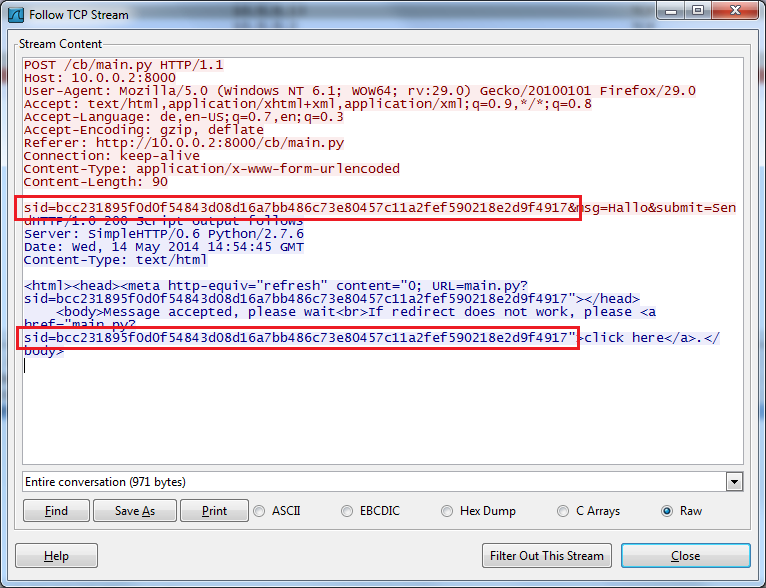
\includegraphics[width=0.8\textwidth]{./imgs/send_message.png}
  }
  \caption{Benutzer schickt eine Message ab}
  \label{fig:message}
\end{figure}
\newline
\newline
Mittels dieser Session-ID erh"alt der Angreifer nun Zugriff auf den Account des Benutzers indem er die gestohlene ID "uber die URL angibt (\lstinline{http://<Server-IP>:8000/cb/main.py?sid=<gestohlene SID des Benutzers>}).

\subsection{Executive summary}
Zusammenfassend lässt sich feststellen, dass aufgrund teilweise schwerwiegender sicherheitsbedingter Mängel der Chatterbox Applikation und fehlender Beachtung im Bezug auf Vertraulichkeit, Integrität und Verfügbarkeit, eine grundlegende Neuprogrammierung von Vorteil wäre.
\section{Lab1b}

\subsection{Sub-Ueberschrift 1}
Lorem ipsum dolor sit amet, consetetur sadipscing elitr, sed diam nonumy eirmod tempor invidunt ut labore et dolore magna aliquyam erat, sed diam voluptua. 

\subsection{Sub-Ueberschrift 2}
Lorem ipsum dolor sit amet, consetetur sadipscing elitr, sed diam nonumy eirmod tempor invidunt ut labore et dolore magna aliquyam erat, sed diam voluptua. At vero eos et accusam et justo duo dolores et ea rebum. 

\subsection{Sub-Ueberschrift 3}
Lorem ipsum dolor sit amet, consetetur sadipscing elitr, sed diam nonumy eirmod tempor invidunt ut labore et dolore magna aliquyam erat, sed diam voluptua. 

\section{Lab1c}

\subsection{Source Code formatieren}
Es folgen einige Beispiele wie Source Code in diesem Dokument formatiert und referenziert werden kann
(\hyperref[code:beispiel1]{siehe Listing~\ref*{code:beispiel1} auf Seite~\pageref*{code:beispiel1}} und \hyperref[code:beispiel2]{siehe Listing~\ref*{code:beispiel2} auf Seite~\pageref*{code:beispiel2}}).

Ebenso können kurzer Code oder kurze Befehle direkt in der Zeile in einem \lstinline{lstinline Block} mit typengleicher Schrift formatiert werden.

\lstinputlisting[caption=Example C/C++ file,label=code:beispiel1,style=c]{example.c}

\begin{lstlisting}[caption=Example bash script,label=code:beispiel2,style=simple]
#!/bin/bash
echo "Bash version ${BASH_VERSION}..."
for i in {0..10..2}
  do
     echo "Welcome $i times"
 done

echo "some very very very very very very very very very very very very very very very very very very very very long string"

exit 0;
\end{lstlisting}

\subsection{Bilder}

Es folgen einige Beispiele wie Bilder in diesem Dokument eingefügt werden können
(\hyperref[fig:logo1]{siehe Abbildung~\ref*{fig:logo1} auf Seite~\pageref*{fig:logo1}}).

\begin{figure}[h!]
  \centering
  \fbox{
    \includegraphics[width=0.4\textwidth]{./imgs/esse-color.png}
  }
  \caption{ESSE Logo}
  \label{fig:logo1}
\end{figure}


%%%%%%%%%%%%%%%%%%%%%%%%%%%%%%%%%%%%%%%%%%%%%%%%%%%%%%%%%%%%%%%%%%%%%%
%
% DO NOT CHANGE THE FOLLOWING PART
%
%%%%%%%%%%%%%%%%%%%%%%%%%%%%%%%%%%%%%%%%%%%%%%%%%%%%%%%%%%%%%%%%%%%%%%

\end{document}


